\documentclass{beamer}

\usepackage[utf8x]{inputenc}
\usepackage{graphicx}
\usepackage{amsthm,amssymb,amsbsy,amsmath,amsfonts,amssymb,amscd}
\usepackage{dsfont}
\usepackage{array}
\newcolumntype{N}{@{}m{2pt}@{}}
\usepackage{tikz}
%\usetikzlibrary{arrows}
%\tikzstyle{block}=[draw opacity=0.7,line width=1.4cm]

\useoutertheme[subsection=false]{miniframes}
\usepackage{lmodern}

\setbeamercolor{author in head/foot}{fg=gray,bg=white}
\setbeamercolor{title in head/foot}{fg=gray,bg=white}
\setbeamercolor{page number in head/foot}{fg=gray,bg=white}
\setbeamercolor{section in head/foot}{bg=black,fg=gray}
\setbeamercolor{subsection in head/foot}{bg=black,fg=gray}

%%%%%%%%%%%%%%%%%%%%%%%%
% GENERAL BEAMER STYLE :

\setbeamertemplate{footline}{
  \hbox{%
    \begin{beamercolorbox}[wd=.2\paperwidth,ht=2ex,dp=1ex,left]{author in head/foot}%
      \hskip1em\usebeamerfont{author in head/foot}\insertshortauthor
    \end{beamercolorbox}%
    \begin{beamercolorbox}[wd=.7\paperwidth,ht=2ex,dp=1ex,center]{title in head/foot}%
      \usebeamerfont{title in head/foot}\insertshorttitle
    \end{beamercolorbox}%
    \begin{beamercolorbox}[wd=.1\paperwidth,ht=2ex,dp=1ex,right]{page number in head/foot}%
      \usebeamerfont{page number in head/foot}\insertframenumber{} / \inserttotalframenumber
      \kern1em 
    \end{beamercolorbox}
  }
}

\setbeamercolor{alerted text}{fg=red!80!black}
\setbeamercolor{itemize/enumerate subbody}{fg=gray!70!black}
\setbeamertemplate{itemize item}[square]
\setbeamertemplate{itemize subitem}[triangle]%{{\textendash}}
\setbeamerfont{itemize/enumerate subbody}{size=\footnotesize}
\setbeamerfont{itemize/enumerate subitem}{size=\footnotesize}

\setbeamertemplate{navigation symbols}{}

\AtBeginSection{
\begin{frame}
    \begin{centering}
    \begin{beamercolorbox}[sep=12pt,center]{part title}
    \usebeamerfont{section title}\insertsection\par
    \end{beamercolorbox}
    \end{centering}
\end{frame}
}

 

\DeclareMathOperator*{\Var}{var}
\DeclareMathOperator*{\E}{E}
\DeclareMathOperator*{\Cov}{cov}
\newcommand\PR[1]{\mathrm{P}\left(#1 \right)}
\newcommand\PS[1]{{\langle #1 \rangle}_\mathcal{H}}
\newcommand\PSi[2]{{ \left \langle #1 \right \rangle}_{\! #2}}
\newcommand\N[1]{{|| #1 ||}_\mathcal{H}}
\newcommand\Ni[2]{{|| #1 ||}_{\! #2}}
\newcommand\dx{\, \mathrm{d}}
\newcommand\textequal{\rule[.4ex]{4pt}{0.4pt}\llap{\rule[.7ex]{4pt}{0.4pt}}}
\newcommand{\argmin}{\operatornamewithlimits{argmin}}
\makeatletter
\newcommand{\shorteq}{%
  \settowidth{\@tempdima}{a}% Width of hyphen
  \resizebox{\@tempdima}{\height}{=}%
}
\makeatother

\title[Majeure Data Science -- Surrogate models and GPR]{\texorpdfstring{ \small Surrogate models and Gaussian Process regression -- lecture 3/5 \\ \vspace{3mm} \LARGE Kriging with trend and/or noisy observations}{}}
\author[Mines St-\'Etienne ]{Mines St-\'Etienne -- Majeure Data Science -- 2016/2017}
\institute{\texorpdfstring{Nicolas Durrande (durrande@emse.fr)}{}}
\date{\null}

%%%%%%%%%%%%%%%%%%%%%%%%%%%%%%%%%%%%%%%%%%%%%%%%%%%%%%
%%%%%%%%%%%%%%%%%%%%%%%%%%%%%%%%%%%%%%%%%%%%%%%%%%%%%%
%%%%%%%%%%%%%%%%%%%%%%%%%%%%%%%%%%%%%%%%%%%%%%%%%%%%%%
\begin{document}

%%%%%%%%%%%%%%%%%%%%%%%%%%%%%%%%%%%%%%%%%%%%%%%%%%%%%%
\begin{frame}
  \titlepage
\end{frame}


%%%%%%%%%%%%%%%%%%%%%%%%%%%%%%%%%%%%%%%%%%%%%%%%%%%%%%
%%%%%%%%%%%%%%%%%%%%%%%%%%%%%%%%%%%%%%%%%%%%%%%%%%%%%%
\section{Approximation}
\subsection{}

%%%%%%%%%%%%%%%%%%%%%%%%%%%%%%%%%%%%%%%%%%%%%%%%%%%%%%
\begin{frame}{}
We are not always interested in models that interpolate the data. For example, if there is some observation noise: $F = f(X) + \varepsilon$.
\begin{center}
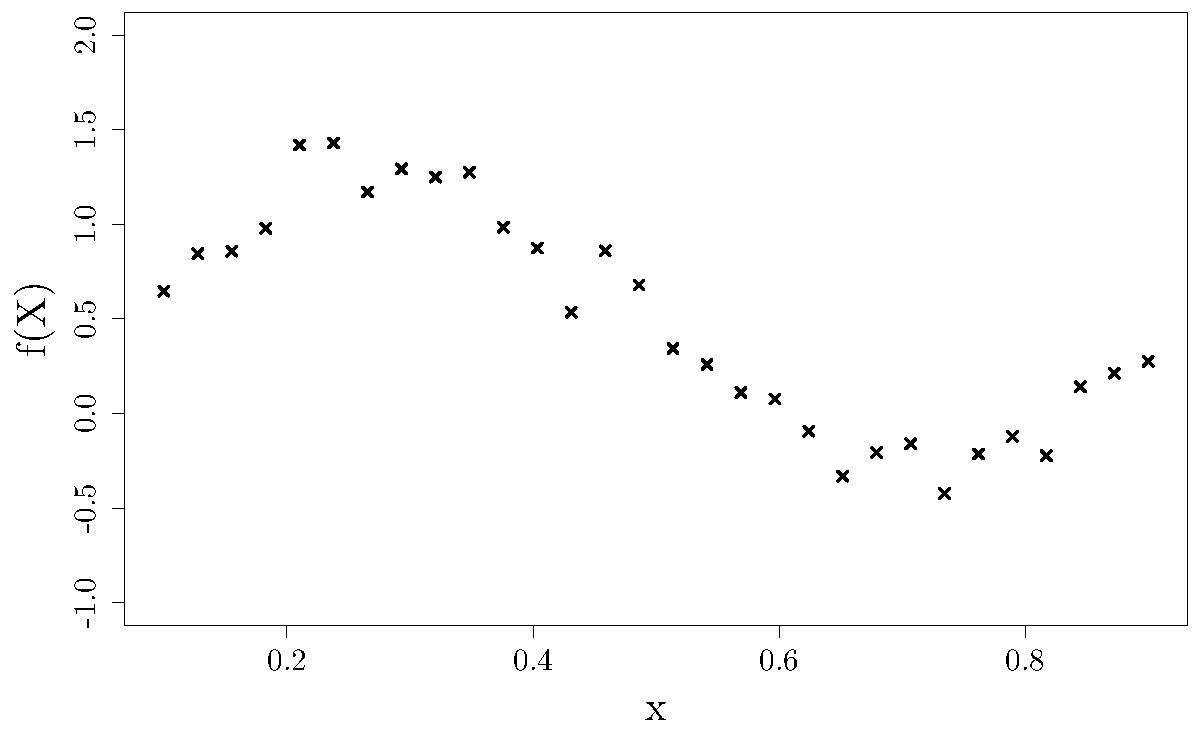
\includegraphics[height=6cm]{figures/R/noisyObs} 
\end{center}
\end{frame}

%%%%%%%%%%%%%%%%%%%%%%%%%%%%%%%%%%%%%%%%%%%%%%%%%%%%%%
\begin{frame}{}
\vspace{5mm}
Let $N$ be a process $\mathcal{N}(0,n)$ that represent the observation noise. The expressions of GPR with noise are 
\begin{equation*}
	\begin{split}
	m(x) &= \E[Z(x)|Z(X) + N(X) \shorteq F] \\
	&= k(x,X) (k(X,X)+n(X,X))^{-1} F \\ 
	& \\
	c(x,y) &= \Cov[Z(x),Z(y)|Z(X)+ N(X) \shorteq F] \\
	&= k(x,y) - k(x,X) (k(X,X)+n(X,X))^{-1} k(X,y)
\end{split}
\end{equation*}
\end{frame}

%%%%%%%%%%%%%%%%%%%%%%%%%%%%%%%%%%%%%%%%%%%%%%%%%%%%%%
\begin{frame}{}
We obtain the following model
\begin{center}
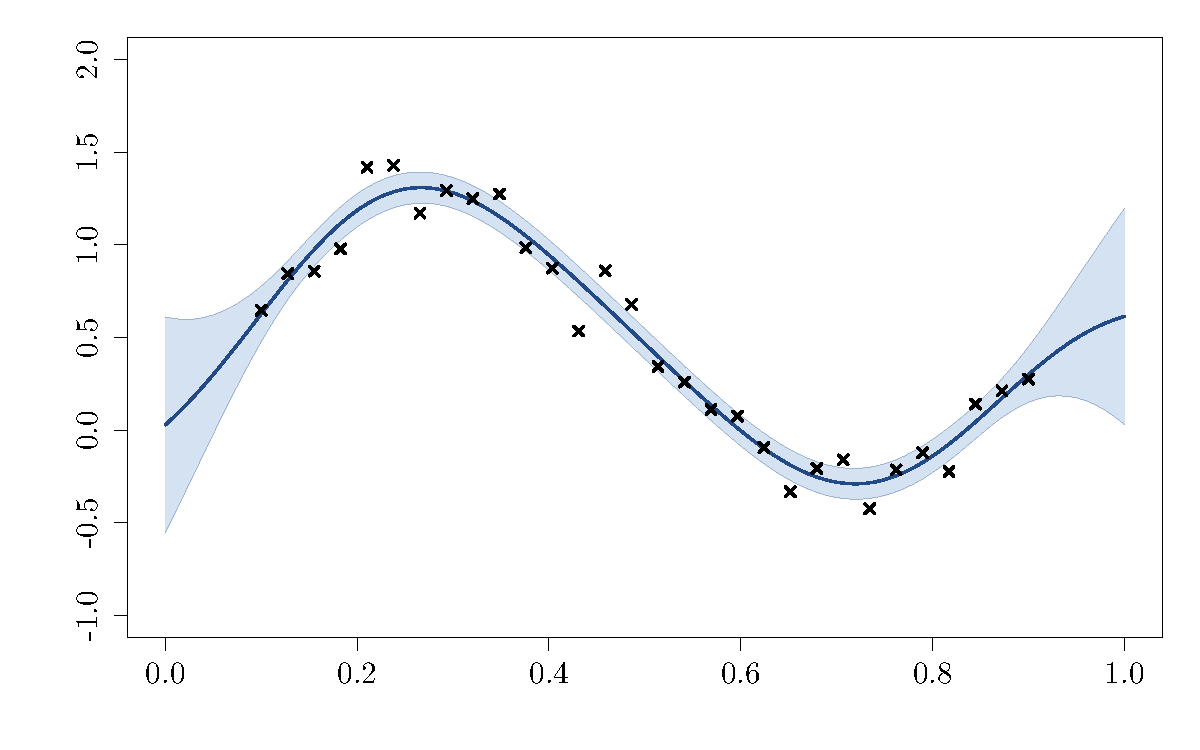
\includegraphics[height=6cm]{figures/R/noisyGPR} 
\end{center}
\end{frame}

%%%%%%%%%%%%%%%%%%%%%%%%%%%%%%%%%%%%%%%%%%%%%%%%%%%%%%
\begin{frame}{}
Influence of observation noise $\tau^2$ (for $n(x,y)=\tau^2 \delta_{x,y}$):
\begin{center}
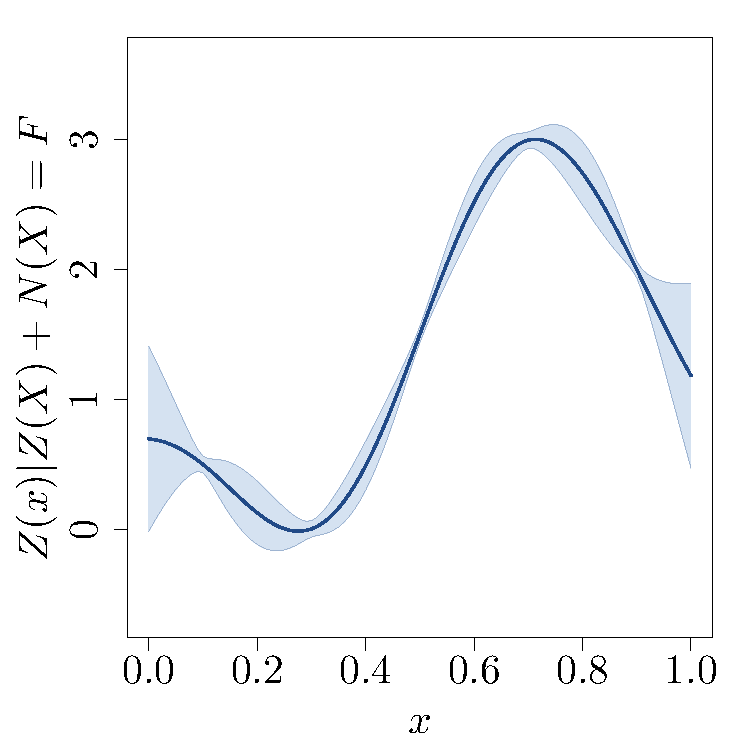
\includegraphics[height=3.5cm]{figures/R/ch34_GPRnoise0001} 
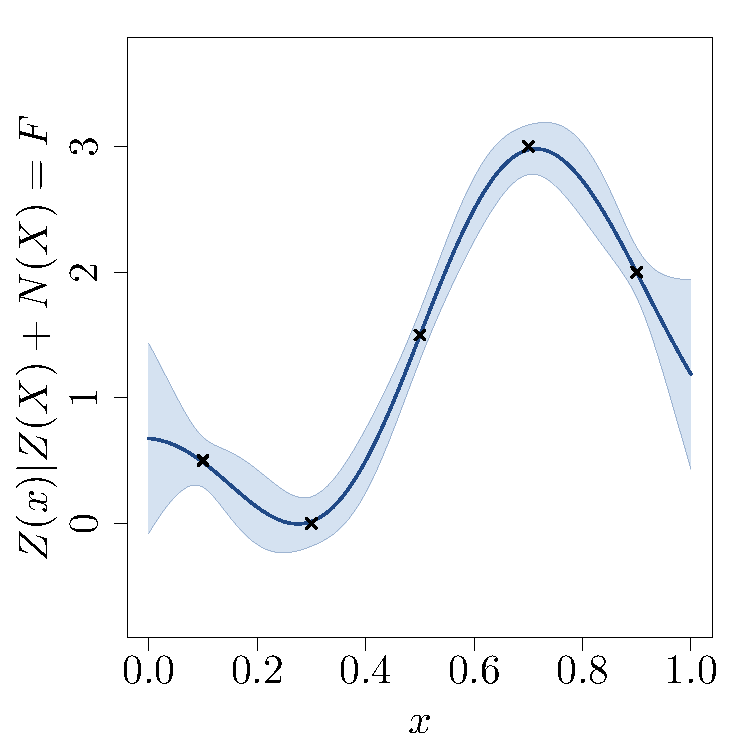
\includegraphics[height=3.5cm]{figures/R/ch34_GPRnoise001} 
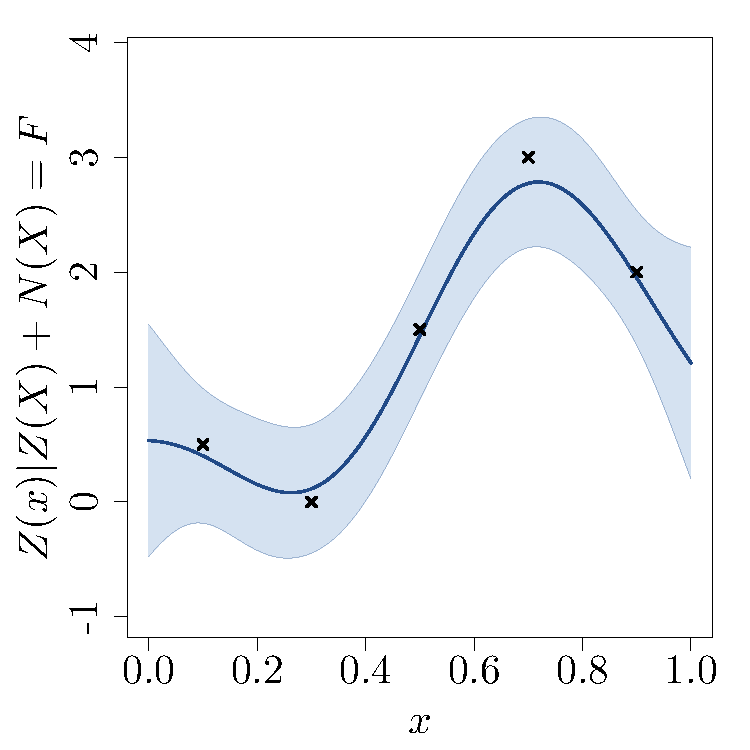
\includegraphics[height=3.5cm]{figures/R/ch34_GPRnoise01}\\
The values of $\tau^2$ are respectively 0.001, 0.01 and 0.1.
\end{center}
In practice, $\tau^2$ can be estimated with Maximum Likelihood. 
\end{frame}




%%%%%%%%%%%%%%%%%%%%%%%%%%%%%%%%%%%%%%%%%%%%%%%%%%%%%%%%%%%%%%%%%%%%%%%%%%%%%%%
%%%%%%%%%%%%%%%%%%%%%%%%%%%%%%%%%%%%%%%%%%%%%%%%%%%%%%%%%%%%%%%%%%%%%%%%%%%%%%%
%%%%%%%%%%%%%%%%%%%%%%%%%%%%%%%%%%%%%%%%%%%%%%%%%%%%%%%%%%%%%%%%%%%%%%%%%%%%%%%
%%%%%%%%%%%%%%%%%%%%%%%%%%%%%%%%%%%%%%%%%%%%%%%%%%%%%%%%%%%%%%%%%%%%%%%%%%%%%%%
\end{document}



\structure{}

\begin{center}
  \begin{tabular}{|c|cc|}

  \end{tabular}
\end{center}

###
%%%%%%%%%%%%%%%%%%%%%%%%%%%%%%%%%%%%%%%%%%%%%%%%%%%%%%
\begin{frame}{}

\end{frame}

###
\begin{block}{}

\end{block}

###
\begin{center}
\includegraphics[height=5cm]{figures/}
\end{center}

###
\begin{columns}[c]
\column{5cm}

\column{5cm}

\end{columns}
